\documentclass{article}

\usepackage{graphicx}
\usepackage{hyperref}
\usepackage{listings}
\usepackage{color}
\usepackage{verbatim}
\usepackage{amsmath}
%\usepackage{subfig}
\usepackage{caption}
\usepackage{subcaption}



\begin{document}
\title{Eric Buras Thesis: Methodology}

\maketitle

\section{Graph Partitioning}
In studying 'small world' networks proposed by Watts and Strogatz \cite{Watts:1998} Fan Chung and Linyuan Lu propose an algorithm that separates a graph into a locally connected component and a global component. Finding a local subgraph is akin to finding a locally connected portion of a graph. Given integers $k \geq 2$ and $l \geq 2$, a $(k,l)$ locally connected graph will have at least $l$ paths connecting any given two nodes with distinct edges in each path. The length of each path can be at most $k$ edges for this pair. A grid network can be described locally with $k=3$ and $l=3$, and is a good example of how a planar graph is connected. Given graph $G$, its maximum locally connected subgraph is the union of all locally connected subgraphs within the entire graph. It is important that this maximum is unique, and can be found through an iterative edge deletion algorithm\cite{Chung:2004}. Search through all edges in the graph, and remove an edge if it does not have at least $l$ edge-disjoint paths of length less than or equal to $k$. Repeat this cycle until no edges can be removed. Chung and Lu prove that this algorithm succeeds regardless of the order of edges removed \cite{Chung:2004}. 

\subsection{Pseudocode}
Given Graph G\\
P = copy(G)\\
While: $Deleted\_edges == True$:\\
\indent Deleted\_edges = False\\
\indent For $edge$ in P.edges:\\
\indent \indent $(start\_node, end\_node) = edge$\\
\indent \indent Search through paths of length $i=2:k$ from $start\_node$ to $end\_node$\\
\indent \indent $count =$  number of edge-disjoint paths\\
\indent \indent if $count \leq l$:\\
\indent \indent \indent P.remove($edge$)\\
\indent \indent \indent $Deleted\_edges = $True\\
	


\begin{figure}
\centering
\begin{subfigure}{.5\textwidth}
  \centering
  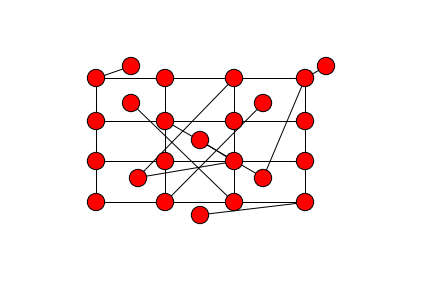
\includegraphics[width=.9\linewidth]{entiregraph.png}
  \caption{Grid with random edges}
  \label{fig:sub1}
\end{subfigure}%
\begin{subfigure}{.5\textwidth}
  \centering
  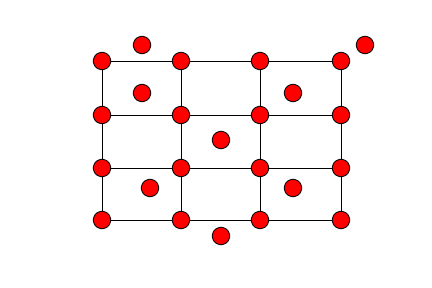
\includegraphics[width=.9\linewidth]{planargraph.png}
  \caption{The planar portion is kept intact}
  \label{fig:sub2}
\end{subfigure}
\caption{Here is a small example of the graph partitioning in action}
\label{fig:test}
\end{figure}

\subsection{NetworkX Library and My Additions}
There is an open source Python library for graph theory and computation called NetworkX written by Hagberg, Schult, and Swart from Los Alamos National Lab. I use many of their functions for reading through edgelists, computing node degrees, converting graphs to Laplacian matrices, etc which are incredibly useful for simple graph work \cite{Hagberg:2008}. Included in this package is a function for creating finding the locally connected subgraph of a graph based upon the work of Chung-Lu above (cite?). Throughout much of the course of my work I used this function to partition my graphs. However for graphs with many edges, this function adds a huge time complexity overhead because it utilizes a shortest path algorithm (cite Dijkstra?). This algorithm should work comparably for any given $k$, $l$ connected subgraphs. However I am focused on $k,l = 3$ so I wrote I an optimized code that simply searches through all potential paths of length 2 and 3 in the graph. This requires much less work than running a shortest path algorithm several thousand times. In the process, and after much debugging and testing, I think that the established NetworkX function has some errors. I now only use my simplified code which speeds up the overall algorithm greatly. Results for partitioning timing are included in the Results section. I hope to work more on my code and submit it as an open-source contribution to the NetworkX package. The established function for partitioning a graph is still important, however, and I hope to work further to find the errors in the function.

\section{Laplacian Solver}
I have partitioned a graph into its locally connected subgraph, $P$ , and the graph of the teleportation edges, $T$. These subgraphs can be converted to Laplacian form with $P_L$ matrix of connections and degree information for the locally connected part, and $T_L$, similar for the teleportation part. With a minor diagonal operation on $T_L$, we have $L = P_L + T_L$ where $L$ is the Laplacian for the entire graph. To solve a Laplacian linear system $Lx=b$ we now solve the two subgraph Laplacians and use linear algebra.

\subsection{Linear Algebra: Woodbury Matrix Identity}
I utilize the Woodbury matrix Identity:\\
\begin{center}
$(A+UCV)^{-1} = A^{-1} - A^{-1}U(C^{-1}+VA^{-1}U)^{-1}VA^{-1}$\\
\end{center}
with A replaced by $P_L$, $U$ and $V$ component matrices of the SVD of $T_L$, and $C$ replaced by a diagonal of the singular values of $T_L$. For a class of graphs we will assume that $P_L$ is very large and sparse, and $T_L$ is very sparse and low rank.

\subsection{Summary of Solving the Laplacian Linear System}
\begin{center}
$Lx=b$\\
$x = L^{-1}b$\\
$x = (P_L+T_L)^{-1}b$\\
$x = (P_L+USV)^{-1}b$\\
Use Woodbury matrix identity\\
$x = (P_L^{-1}-P_L^{-1}U(S^{-1}+VP_L^{-1}U)^{-1}VP_L^{-1})b$\\
$x = P_L^{-1}b-P_L^{-1}U(S^{-1}+VP_L^{-1}U)^{-1}VP_L^{-1}b$\\
\end{center}


\subsection{Algebraic Multigrid of Locally Connected Subgraph}
The locally connected subgraph is planar, meaning it can be drawn on a piece of paper without any edges crossing (proof it is planar?). Using work beginning with Gary Miller \cite{Miller:1995}, we know that an Algebraic Multigrid solver is optimal for this planar graph laplacian matrix as the solution space is split into multiple cycles of coarsened solving \cite{Brandt:1984}. Previous approaches to using multigrid (LAMG, CMG, Cascadic) to solve Laplacian linear systems do not have a systematic method of graph coarsening. They are based on heuristics for identifying which edges to keep in the multiple levels. Whereas these algorithms are prone to losing edge information in the multiple coarsening cycles, my algorithm runs multigrid only on the planar portion, preserving correct edge information in the coarse levels. (do i need to cite?)There are many multigrid solves in this algorithm, and it is important to optimize performance. Thus I use the Portable, Extensible Toolkit for Scientific Computation (PETSc) and its python library petsc4py to run multigrid solves \cite{petsc-user-ref, Dalcin:2011}

\subsection{Low Rank SVD of Teleportation Subgraph}
For graphs I am interested in, the number of edges in the Teleportation subgraph is very small relative to the size of the original graph. This causes the laplacian matrix of teleportation subgraph, $T_L$, to have very low rank structure. I can then take the low rank singular value decomposition (cite?) to solve this small portion. Given $nxn$ matrix $T_L$ with rank $r$, we compute $USV = T_L$ where $T_L$ has $r$ non-negligible singular values. Thus U is tall-skinny $nxr$, S is an $rxr$ diagonal matrix of the non-negligible singular values, and V is short-fat $rxn$. This low-rank SVD is also important in decreasing the floating point operations in the matrix-matrix, and matrix-vector operations.









\bibliographystyle{plain}
\bibliography{mastersbib}
\end{document}